% -----------------------------------------------------------------------------
% Fundamentação Teórica
% -----------------------------------------------------------------------------

\chapter{Fundamentação Teórica}
\label{chap:fundamentacaoTeorica}

O presente capítulo tem como objetivo discutir a teoria por trás do \textit{design system}. O capítulo é introduzido conceituando a idéia de \textit{design} de interação, apresentando o contexto do seu surgimento e os desafios que ele traz consigo. Logo em seguida, é discutida a questão da experiência do usuário no mercado de software moderno. Finaliza-se o capítulo, dissecando o \textit{design system} e por fim apresentando o \textit{atomic design} como proposta de metodologia para sua implementação.

\section{Design de Interação}
\label{sec:designInteracao}

Nos primórdios da era da computação, os primeiros sistemas computacionais eram criados para atender demandas dos próprios engenheiros que os criavam, ou eram destinados à usuários com um background técnico muito avançado. As interfaces com os computadores da época eram, em geral, baseadas em painéis com chaves e componentes que indicavam o estado atual dos circuitos internos do sistema (LEDs). Restava ao usuário final apenas uma extensa documentação a ser lida, de forma a de fato entender o comportamento do sistema \cite{preece2005design}.

Foi no final dos anos 70 e início dos anos 80, com o advento dos monitores e estações de trabalhos pessoais, que o design de interface passou a existir \cite{grudin1990computer}. Um dos principais desafios da época foi o desenvolvimento de sistemas acessíveis à pessoas comuns, de forma a auxiliá-las a desenvolver tarefas intelectuais simples, como escrever documentos por exemplo \cite{preece2005design}.

Para tornar isso possível, reuniram-se profissionais de diferentes áreas para estudar as novas possibilidades que o design de interface de usuários trazia consigo. Cientistas da computação, psicólogos, designers gráficos e designers de produtos uniram seus esforços para o estudo e desenvolvimento de interfaces gráficas (abreviadas GUI), de forma a atender à demanda latente por esse tipo de sistema. Nessa época muitos estudos foram feitos na área de design de produtos, com o intuito de entender a melhor maneira de estruturar os diferentes componentes visuais do sistema na interface de usuário \cite{preece2005design}.

Atualmente, segundo \cite{preece2005design}, entende-se como design de interação:
“Design de produtos interativos que fornecem suporte às atividades cotidianas das pessoas, seja no lar ou no trabalho. Significa criar experiências que melhoram e estendem a maneira como as pessoas trabalham, se comunicam e interagem”. 
O autor ainda faz uma breve analogia, embasado em Terry Winograd, ao descrever o design de interação. A analogia tem como base o questionamento das diferenças de pensamento entre arquitetos e engenheiros ao se depararem com o mesmo problema de se construir uma casa. O autor pondera que, o trabalho do arquiteto muito se assemelha à de um designer, com um caráter artístico, mais voltado para a usabilidade. Por outro lado, o engenheiro é associado ao desenvolvedor de software, com características bastante técnicas. Apesar de ser um um ponto de vista válido, o objetivo do presente trabalho é justamente questionar esse modelo de visão segregatória do mercado, onde os papéis de designers e desenvolvedores estão muitas vezes isolados. Deve-se haver uma linguagem comum entre designers e desenvolvedores, que proporcione uma rica troca de idéias entre os diferentes tipos de profissionais e garanta os benefícios de se ter times realmente multidisciplinares. A linguagem proposta para esse problema é o que se entende como \textit{Design System}.

\section{Experiência do usuário e o mercado de desenvolvimento de software moderno}
\label{experienciaUsuarioMercado}

O design de interação com foco no usuário final nasceu em um formato de estudos de usabilidades nos anos 70 e 80 \cite{gould1985designing, nielsen1994usability}. Algum tempo depois, já nos anos 2000, a metódologia de \textit{design thinking} começou a ganhar espaço no mercado como meio de inovação em empresas de tecnologias \cite{martin2009design}. Entretando, mesmo após avanços literários na área de design, o que se percebe no dia-a-dia das empresas de tecnologia da atualidade é algo bastante diferente daquilo pregado pela academia:  o design é, muitas vezes, negligenciado no processo de desenvolvimento de software \cite{winograd1996bringing}.

Com o advento das metodologias de desenvolvimento ágil, no início dos anos 2000, o mercado de desenvolvimento de software passou por drásticas alterações em seus processos internos. O resultado dessas mudanças foi, em geral, um aumento na taxa de projetos bem sucedidos e da satisfação dos seus \textit{stakeholders} \cite{serrador2015does}. Todavia, enquanto a experiência do usuário vinha se tornando diferencial no mercado, sua reflexão acaba sendo postergada para o final das iterações da maioria dos processos ágeis, como o Scrum por exemplo \cite{ruissalo2018operating}.

A inclusão do designer em times ágeis, os forçando à cumprir as mesmas agendas e ritos propostos pelo processo, além de se mostrar ineficaz ao entender a real necessidade do usuário, também conduz a organização para um crescente legado de design em seu produto \cite{ruissalo2018operating}. Portando, mesmo que processos ágeis sejam mais lucrativos do que o modelo de desenvolvimento em cascata vivenciado por gerações de software anteriores, a experiência do usuário no desenvolvimento de software se torna míope, dada as agendas de \textit{sprints} que os designers acabam sendo submetidos.

De fato, a inclusão do design como parte do processo de desenvolvimento e da cultura de uma empresa é uma tarefa desafiadora. Dessa forma, para entender os problemas e a maturidade em design das organiações \cite{nielsen1994usability} criou um modelo de maturidade em experiência do usuário, ilustrado pelo \autoref{table:uxMaturity}.

\begin{quadro}[!htb]
\centering
\begin{tabular}{|m{5cm}|m{9cm}|} \hline
	
	\multicolumn{1}{|c|}{\bfseries Estágio de Maturidade} & \multicolumn{1}{c|}{\bfseries Características} \\\hline
	
	 1: Hostil & Desenvolvedores simplesmente não querem saber dos usuários e suas necessidades \\\hline
	 
	 2: Centrada no desenvolvedor & Time toma decisões de acordo com suas intuições \\\hline
	 
	 3: Embrionária & Pesquisas de guerrilha ou consulta única à poucos usuários \\\hline
	 
	 4: Orçamento dedicado & Atividades de UX são planejadas \\\hline
	 
	 5: Gerenciada & Existe oficialmente um grupo de UX, gerenciado por um gerente que pensa na experiência do usuário para a organização \\\hline
	 
	 6: Processo sistemático & Qualidade de UX é acompanhada e existe um processo de criação interativo \\\hline
	 
	 7: Integrada & A organização emprega os dados de usuários como diretriz para se decidir o quê e como contruir novas funcionalidades \\\hline
	 
	 8: Empresa orientada ao usuário & Os dados de usuários guiam as estratégias da empresa \\\hline
    
\end{tabular}
\caption{Maturidade em experiência do usuário (UX)}
\label{table:uxMaturity}
\fonte{\citeonline{nielsen1994usability}}
\end{quadro}

Em complemento à \cite{nielsen1994usability}, \cite{curtis2010modular} considera a linguagem de comunicação entre os times de UX e desenvolvimento como parte da maturidade em design de uma organização. Segundo ele, desenvolvedores e designers normalmente utilizam diferentes termos para os mesmos conceitos relacionados à software.

\section{\textit{Design System}}
\label{sec:designSystem}

 \begin{quote}{Alex Schleifer, VP of Design (Airbnb)}
  \textit{You can’t innovate on products without first innovating the way you build them.}
 \end{quote}
 
Conforme as organizações e seus produtos vão evoluindo, começam a surgir problemas de escalabilidade em design e desenvolvimento \textit{frontend} \cite{curtis2010modular}:

\begin{itemize}
  \item Guias de estilo se tornam desatualizados facilmente, uma vez que não existe ligação alguma com o código-fonte do produto. Além disso, podem se mostrar bastante verbosos e extensos, o que vai de encontro com a produtividade.
  \item Designers e desenvolvedores acabam reinventado solução já desenvolvidas em outros projetos, causando incosistências no produto.
\end{itemize}

Nesse contexto, surge-se o conceito de \textit{Design System} como artefato que aumeja sanar os problemas listados acima, unificando guias de estilo e bibliotecas de componentes em um mesmo ambiente, de maneira prática e sistemática. Dessa forma, consitência e reusabilidade no produto, além de uma boa comunicação entre desenvolvedores e designer podem ser conquistadas \cite{curtis2010modular}.

Para melhorar a eficiência e consistência das interfaces de usuários criadas para seus produtos, o \textit{design system} traz consigo os seguites artefatos \cite{ruissalo2018operating}:

\begin{itemize}
  \item Princípios de design
  \item Guia de tom de voz
  \item Biblioteca de componentes
\end{itemize}

\subsection{Princípios de \textit{design}}

Formando a espinha dorsal do design, os princípios fornecem uma base comum para os times de uma organização no processo de tomada de decisão em problemas de design. Eles são baseados principalmente nos valores da empresa e são aplicados claramente na forma como se conduz a experiência do usuário e na criação de interfaces de usuário. Princípios de \textit{design} podem dar direção na forma como o departamento de marketing se comunica, podem focar em termos de cultura do time, ou até mesmo no processo de design como um todo \cite{kholmatova2017design}.

Para ilustrar a maneira como os princípios de \textit{design} são adotados na indústrica, serão apresentados dois exemplos reais de grandes empresas da atualidade: Mongodb e Pluralsight.

Primeiramente, a Mongodb, empresa que mantém um banco de dados não-relacional como principal produto, optou por definir seus princípios de forma a englobar tanto diretrizes de produto como de cultura. O \autoref{table:mongodbDesignPrinciples} e a \autoref{fig:mongodbDesignPrinciples} apresentam o modelo utilizado pela empresa.


\begin{figure}[!htb]
	\centering
	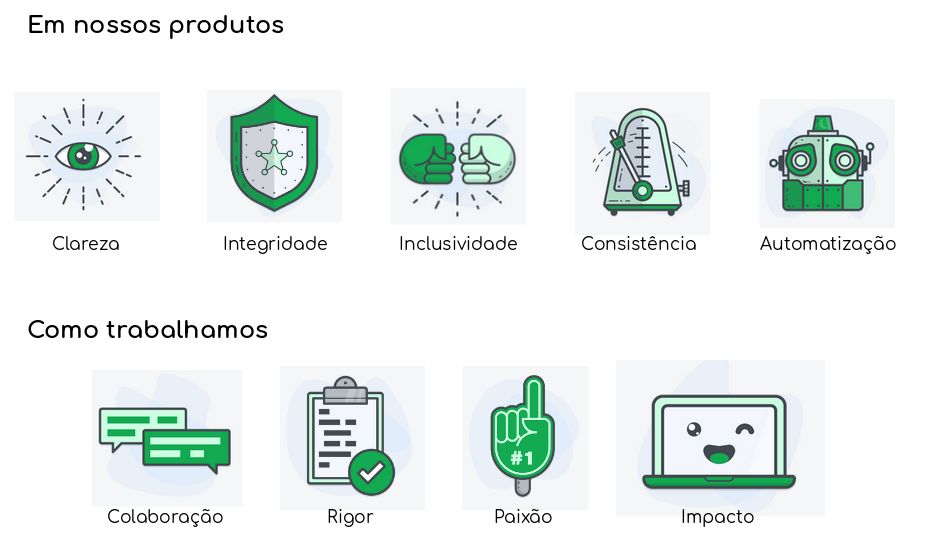
\includegraphics[width=\linewidth]{./04-figuras/02_referencial_teorico/mongodb-design-principles.png}
	\caption{Princípios de \textit{design} da Mongodb}
  \label{fig:mongodbDesignPrinciples}
\end{figure}

\begin{quadro}[!htb]
	\centering
	\begin{tabular}{|m{2cm}|m{12cm}|} \hline
		
		\multicolumn{1}{|c|}{\bfseries Princípio de \textit{Design}} & \multicolumn{1}{c|}{\bfseries Descrição} \\\hline
		
		 Clareza & Através do uso de padrões familiares, fluxos de trabalho guiados, instruções em linha e informações contextuais, nossos produtos são compreendidos sem a necessidade de um manual, quando possível, e fornecem acesso fácil à documentação concisa e clara onde necessário. A terminologia é cuidadosamente considerada e mapeia de perto o propósito ou conceito que descreve. \\\hline
		 
		 Integridade & As informações comunicadas ao usuário são precisas e completas. A transparência total instiga confiança na resiliência e segurança do produto, o que é crucial para o gerenciamento de infraestrutura crítica \\\hline
		 
		 Inclusividade & Nossos produtos atendem a todos, desde iniciantes que aprendem a usar o MongoDB pela primeira vez para especialistas na área. Quando um iniciante se sente preso, o produto fornece orientação. Quando um especialista deseja um atalho ou recurso avançado, o produto o fornece exatamente como o usuário esperaria. \\\hline
		 
		 Consistência & Os padrões de informação e interação que aparecem em diferentes lugares são consistentes visualmente e conceitualmente. Isso permite que os usuários movam-se com fluidez através de nossos produtos, confiantes de que o que aprenderem em um deles será transferido para todos os outros. \\\hline
		 
		 Automatização & Nossos produtos transmitem uma compreensão de que, às vezes, o melhor design é invisível para o usuário. Quando automatizamos uma tarefa, reduzimos a chance de erro do usuário, levando a uma experiência geral mais segura. Nossos produtos automatizam quando possível, deixando o controle com o usuário quando necessário \\\hline
		 
		 Colaboração & Reconhecemos que o melhor trabalho vem da colaboração diligente. Trabalhamos lado a lado com outros designers, engenheiros e gerentes de produto. \\\hline
		 
		 Rigor & Não estamos satisfeitos com nossas soluções até que as testamos e comprovamos sua eficácia. Nós validamos idéias e conceitos no início do processo de design, antes que qualquer \textit{wireframing} ocorra. Dados é o que nos guia. \\\hline
		 
		 Paixão & Somos intensamente apaixonados pelo nosso trabalho. Nós nos esforçamos para um nível de excelência que encanta o usuário. Mesmo detalhes aparentemente imperceptíveis recebem atenção especial. \\\hline
		 
		 Impacto & Valorizamos o impacto nas nossas entregas. Reconhecemos que nossas ferramentas e processos, enquanto evoluindo e melhorando constantemente, são apenas um meio de alcançar resultados positivos para o usuário. \\\hline
			
	\end{tabular}
	\caption{Princípios de \textit{design} da Mongodb}
	\label{table:mongodbDesignPrinciples}
\end{quadro}

Por outro lado, a Pluralsight, uma das maiores plataformas de cursos online de tecnologia da atualidade, definiu seus princípios de forma a guiar a maneira como se comunica com seu público alvo. A \autoref{fig:pluralsightDesignPrinciples} detalha tais princípios.

\begin{figure}
	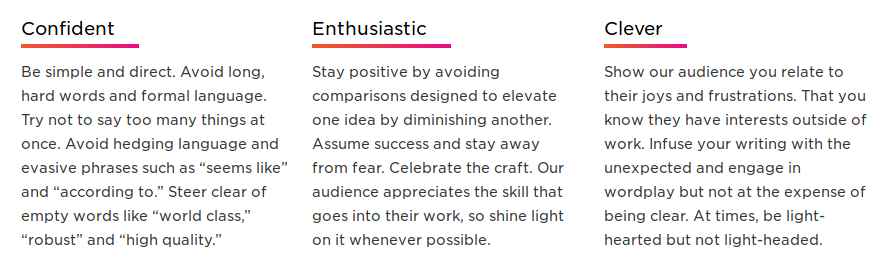
\includegraphics[width=\linewidth]{./04-figuras/02_referencial_teorico/pluralsight-principles.png}
	\caption{Princípios de \textit{design} da Pluralsight}
	\fonte{\citeonline{pluralsightDesignPrinciples}}
  \label{fig:pluralsightDesignPrinciples}
\end{figure}

Percebe-se, dados os dois exemplos apresentados, que a abordagem adotada pelas empresas na definição dos seus princípios pode variar. Não existe consenso em qual aspecto a organização deve focar. Cada empresa tem seu próprio contexto e cabe a ela aplicar os princípios da melhor maneira possível \cite{kholmatova2017design}.

Princípios de \textit{design} devem ser relacionáveis uns aos outros, fáceis de se lembrar e limitados em número. Em contrapartida, devem ser específicos o suficiente para serem capazes de auxiliarem os designers a tomarem decisões e julgar opções de maneira consistente \cite{kholmatova2017design}.

\subsection{Tom de voz}
\label{subsec:tomVoz}

No domínio verbal, os guias de tom de voz ajudam a definir a maneira com que uma organização se comunica com seu público alvo \cite{ruissalo2018operating}.

De acordo com \cite{impactOfVoiceTone}, o tom de voz tem grande impacto na percepção de confiabilidade, amigabilidade e desejo dos usuários em relação aos produtos e serviços de uma empresa. Dado que grandes organizações podem ter vários times internos, uma guia de tom de voz é fundamental para dar diretriz aos times, de forma a garantir uma comunicação coesa e consistente entre a empresa e seus clientes. \cite{impactOfVoiceTone} categoriza o tom de voz em quatro dimensões: engraçada \textit{vs} séria, casual \textit{vs} formal, insolente \textit{vs} respeitosa, entusiástica \textit{vs} objetiva.

A Firefox, empresa que mantém um navegador para internet como produto, utilizou a categorização proposta por \cite{impactOfVoiceTone}. Como pode ser visto pelas figuras \ref{fig:firefoxVoiceToneSerious} e \ref{fig:firefoxVoiceTonePlayful}, existem diferenças na maneira como a empresa se comunica com seus usuários dependendo das circunstâncias. Para situações onde ajudar o usuário é prioridade, como em casos de erros, o tom de voz é mais sério. Por outro lado, em situações onde o objetivo é motivar o usuário a tomar alguma ação -- como \textit{onboarding}, sincronização de dados ou \textit{login} -- o tom de voz é mais descontraído, não deixando de ser respeitoso.

\begin{figure}
	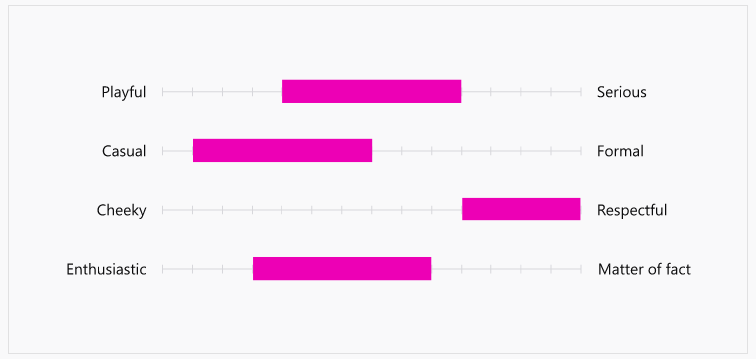
\includegraphics[width=\linewidth]{./04-figuras/02_referencial_teorico/firefox-tone-voice-01.png}
	\caption{Tom de voz para mensagens de suporte críticas da Firefox}
	\fonte{\citeonline{firefoxVoiceTone}}
  \label{fig:firefoxVoiceToneSerious}
\end{figure}

\begin{figure}
	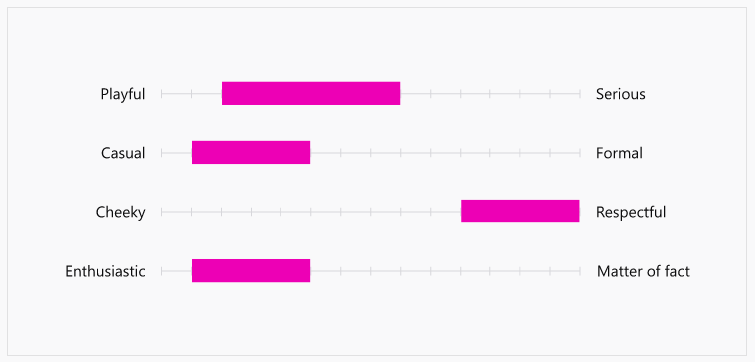
\includegraphics[width=\linewidth]{./04-figuras/02_referencial_teorico/firefox-tone-voice-02.png}
	\caption{Tom de voz para mensagens motivacionais da Firefox}
	\fonte{\citeonline{firefoxVoiceTone}}
  \label{fig:firefoxVoiceTonePlayful}
\end{figure}

\subsection{Biblioteca de componentes}
\label{sec:bibliotecaComponentes}

Desde a concepção das interfaces de usuário (GUI), a relevância da consistência nas interfaces através dos diferentes produtos de uma organização foi percebida imediatamente \cite{ruissalo2018operating}. Para sanar esse problema, foi proposta a definição das chamadas bibliotecas de componentes. A \autoref{fig:bootstrapStyleGuide} apresenta um exemplo de biblioteca de componentes muito utilizada pela indústria: Bootstrap.

As bibliotecas de componentes tradicionais eram focadas em padronizar o uso dos componentes do produto, como tipografia, imagens e ilustrações, cores, \textit{layouts} e outros elementos gráficos \cite{ruissalo2018operating}. Eram, portanto, focadas somente nos aspectos visuais das aplicações, definindo o que era esperado a ser apresentado para o usuário final.

De acordo com \cite{taylor2007software}, \textit{design} no contexto de desenvolvimento de software está mais diretamente ligado na arquitetura dos produtos ao invés de uma mero padrão de estilização. Essa é a razão pela qual o \textit{design} pode, e deve, estar mais próximo da implementação do \textit{software}. Tal abordagem vai de encontro com um antigo dogma: guias de estilo e bibliotecas de componente são propriedade dos \textit{designers} \cite{ruissalo2018operating}. Espera-se que as bibliotecas de componentes sejam o resultado do trabalho conjunto de \textit{designers} e desenvolvedores.

\begin{figure}
	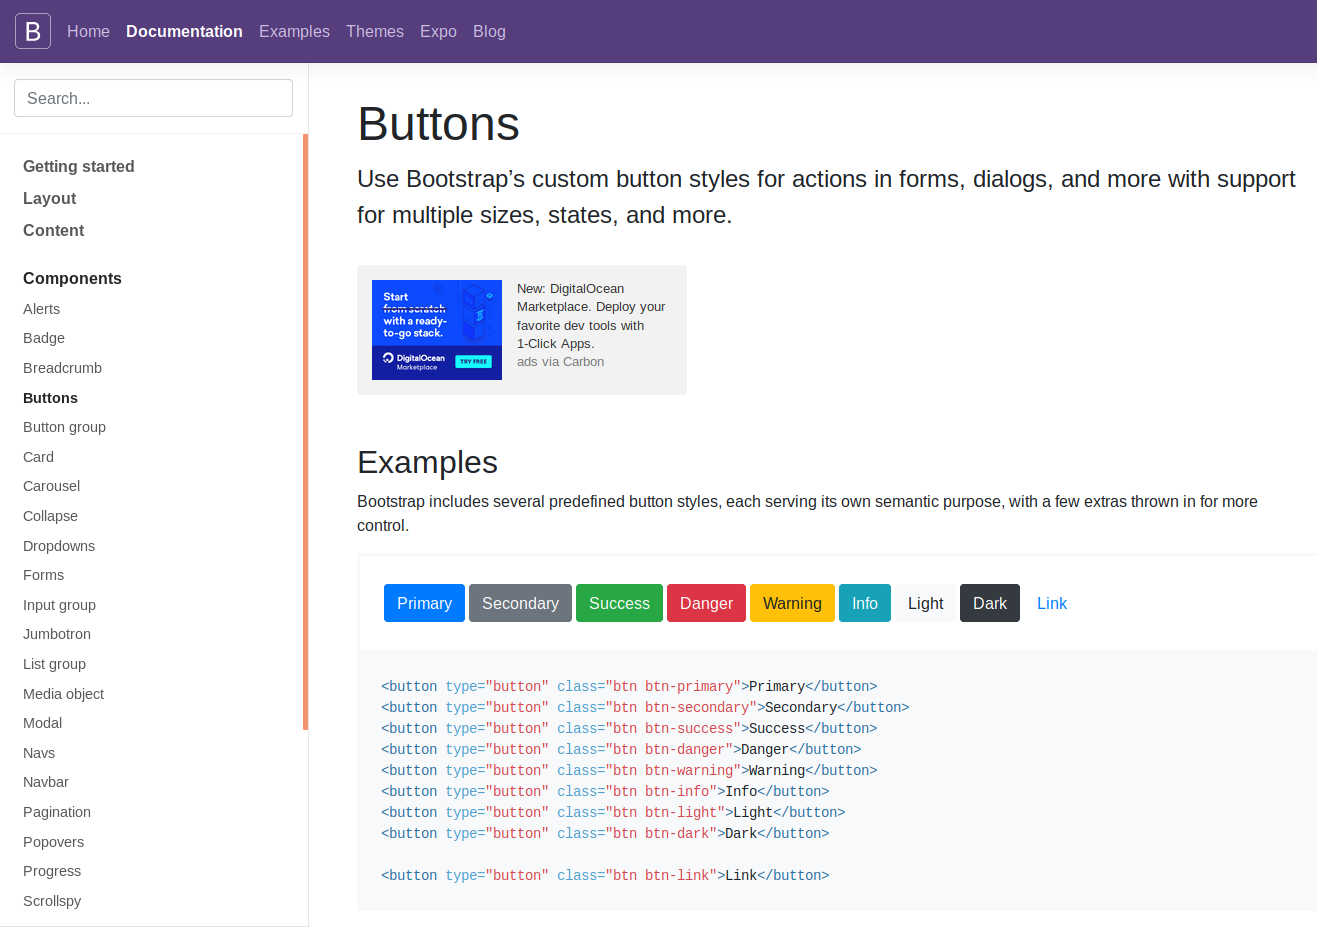
\includegraphics[width=\linewidth]{./04-figuras/02_referencial_teorico/bootstrap.png}
	\caption{Exemplo de biblioteca de componentes}
	\fonte{\citeonline{bootstrapStyleGuide}}
  \label{fig:bootstrapStyleGuide}
\end{figure}

\section{\textit{Atomic Design}}
\label{sec:atomicDesign}

Conforme apresentado na seção anterior, \textit{Design Systems} se propõem a revolucionar a forma como se constroi interfaces de usuário à nível profissional. Entretanto, a forma como são apresentados seus conceitos é, em geral, um tanto quanto subjetiva, ficando a cargo de cada instituição definir a melhor abordagem para o seu problema. Para o caso das bibliotecas de componentes em especial, tanta liberdade assim poderia acarretar em problemas de escalabilidade da solução.

Com o intuito de definir uma metodologia para a implementação técnica de um \textit{Design System}, \cite{frostAtomicDesign} buscou na química inspiração para a resolução do problema. A idéia residia no fato de que toda matéria -- seja sólida, líquida, gasosa, simples, complexa, etc -- é composta por unidades minúsculas e indivisíveis (ou quase) chamadas átomos. Tais átomos, combinados entre si formam unidades mais complexas, conhecidas como moléculas. Essas, por sua vez, combinadas formas estruturas ainda mais complexas chamadas organismos. E assim é expressa toda a mateŕia do universo.

Analogamente à matéria, interfaces de usuários também podem ser expressas por componentes menores. Isso significa que é possível construir interfaces bastante complexas através de um conjunto de componentes menores e mais simples. A \autoref{fig:periodicTable} ilustra e categoriza elementos HTML a níveis atômicos.

\begin{figure}
	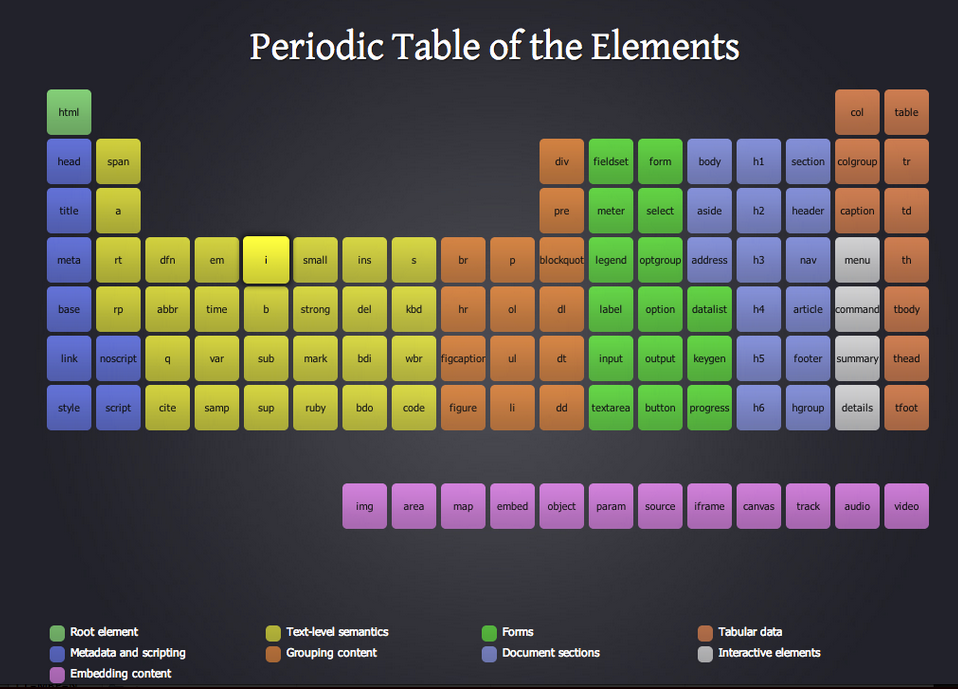
\includegraphics[width=\linewidth]{./04-figuras/02_referencial_teorico/periodic-table.png}
	\caption{Tabela períodica de elementos HTML proposta por Josh Duck}
	\fonte{\citeonline{frostAtomicDesign}}
  \label{fig:periodicTable}
\end{figure}

Dessa forma, \cite{frostAtomicDesign} defende a existência de cinco níveis distintos no \textit{Atomic Design}: Átomos, Moléculas, Organismos, Templates e Páginas. A \autoref{fig:atomicDesignLevels} ilustra tais níveis e a forma como eles comunicam entre si.

\begin{figure}
	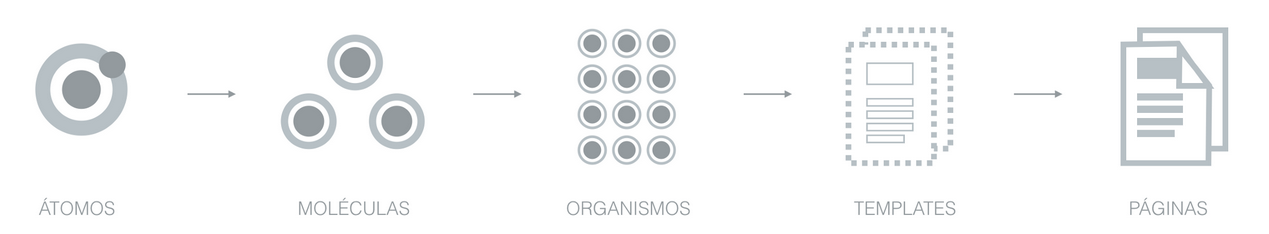
\includegraphics[width=\linewidth]{./04-figuras/02_referencial_teorico/atomic-levels.png}
	\caption{Níveis do \textit{Atomic Design}}
	\fonte{\citeonline{frostAtomicDesign}}
  \label{fig:atomicDesignLevels}
\end{figure}

\subsection{Átomos}
\label{subsec:atomos}

Átomos são os blocos básicos para construção da matéria. Aplicados no universo de interfaces de usuário Web, átomos são as \textit{tags} HTML, como um \textit{input}, botão, \textit{label}, etc.

Assim como os átomos da natureza, eles não são muito úteis de serem manipulados individualmente. Entetanto, cumprem um papel fundamental na construção da biblioteca de componentes, uma vez que todos os componentes mais complexos do sistema são construídos com base neles.

\subsection{Moléculas}
\label{subsec:moleculas}

Tudo começa a ficar mais tangível quando combinamos átomos. As moléculas são um conjunto de átomos distintos que ficam encapsulados juntos. São a espinha dorsal de todo o \textit{Design System}.

Por exemplo, um \textit{label}, um botão e um \textit{input} individualmente não são muito úteis para o usuário final, porém juntos eles formam um formulário que pode de fato gerar valor para o interlocutor.

Construir moléculas a partir de átomos estimula os desenvolvedores a seguir a mentalidade de "faça uma vez, mas faça direito" \cite{frostAtomicDesign}.

\subsection{Organismos}
\label{subsec:organismos}

Organismos são grupos de moléculas que juntas formam uma seção relativamente complexa e distinta da interface de usuário. Examplos de organismos poderiam ser: o cabeçalho de uma página, a seção de menu, etc.

Como organismos já estão em um nível bastante concreto, conseguem definir a estrutura da interface do usuário com bastante clareza. São comumente utilizados como base para uma conversa com clientes finais de um dado produto, uma vez que conseguem transmitir a idéia de valor de uma funcionalidade.

Construir organismos a partir de moléculas estimula os desenvolvedores a construir componentes portáveis e reusáveis \cite{frostAtomicDesign}.

\subsection{Templates}
\label{subsec:templates}

Chegando no nível de templates, abre-se mão da analogia à química para se valorizar uma linguagem que faça mais sentido para os clientes da aplicação. Templates consistem em um conjunto de organismos que compõem uma página. Aqui, começa-se a visualizar o resultado final do \textit{design}, podendo-se visualizar o \textit{layout} em ação.

A \autoref{fig:atomicDesignTemplate} apresenta um exemplo de um possível template em um \textit{Atomic Design}.

\begin{figure}
	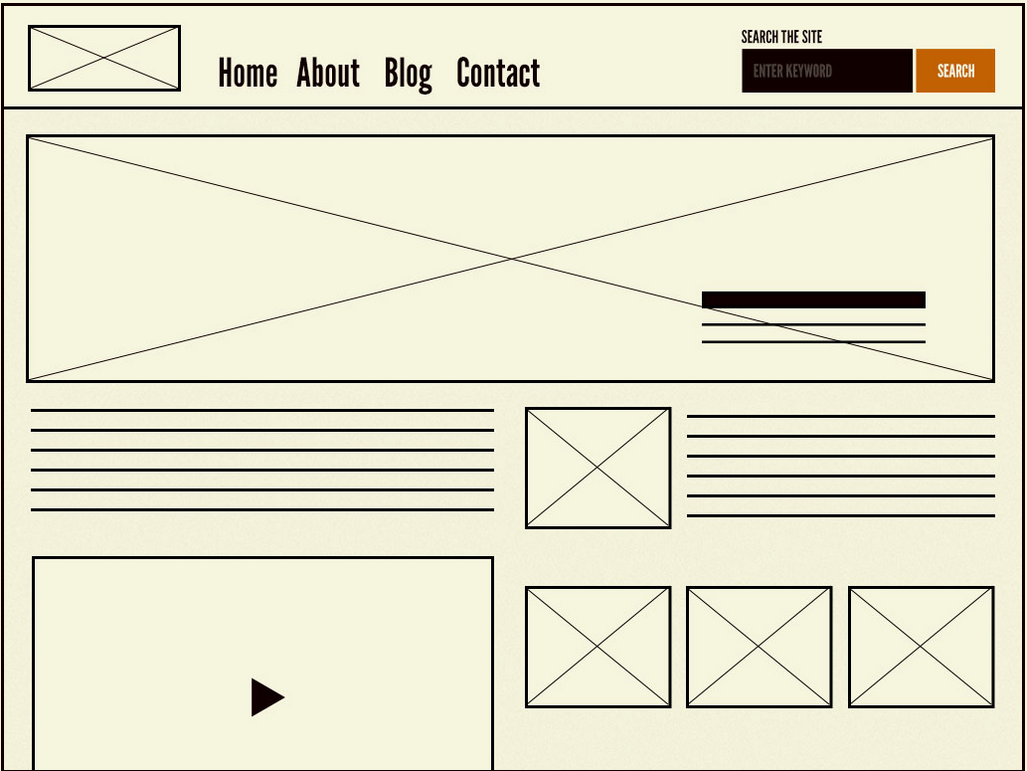
\includegraphics[width=\linewidth]{./04-figuras/02_referencial_teorico/ad-template.png}
	\caption{Exemplo de template}
	\fonte{\citeonline{frostAtomicDesign}}
  \label{fig:atomicDesignTemplate}
\end{figure}

\subsection{Páginas}

Páginas são instâncias específicas de um dado template. Nesse momento, conteúdos de marcação são substituídos por valores reais a serem utilizados na interface de usuário.

Esse estágio é crucial pois é nele onde se testa a efetividade do \textit{design system}. Visualizando todos componentes em um mesmo ambiente facilita o trabalho de validar e eventualmente modificar algum átomo, mólecula, organismo ou template, de forma a atingir melhores resultados.
